% Single-file Overleaf version.
% Just replace main.tex content with this file's content, then Recompile.
% No need to upload references.bib separately -- it is embedded via filecontents.

\begin{filecontents*}[overwrite]{references.bib}
@article{su2021roformer,
  title={{RoFormer: Enhanced Transformer with Rotary Position Embedding}},
  author={Su, Jianlin and Lu, Yu and Pan, Shengfeng and Wen, Bo and Liu, Yunfeng},
  journal={arXiv preprint arXiv:2104.09864},
  year={2021}
}

@inproceedings{kwon2023vllm,
  title={{Efficient Memory Management for Large Language Model Serving with PagedAttention}},
  author={Kwon, Woosuk and Li, Zhuohan and Zhuang, Siyuan and Sheng, Ying and Zheng, Lianmin and Yu, Cody Hao and Gonzalez, Joseph E. and Zhang, Hao and Stoica, Ion},
  booktitle={SOSP},
  year={2023}
}

@inproceedings{zheng2024sglang,
  title={{SGLang: Efficient Execution of Structured Language Model Programs}},
  author={Zheng, Lianmin and Yin, Liangsheng and Xie, Zhiqiang and Sun, Chuyue and Huang, Jeff and Yu, Cody Hao and Cao, Shiyi and Kozyrakis, Christos and Stoica, Ion and Gonzalez, Joseph E. and others},
  booktitle={NeurIPS},
  year={2024}
}

@article{gim2023prompt,
  title={{Prompt Cache: Modular Attention Reuse for Low-Latency Inference}},
  author={Gim, In and Chen, Guojun and Lee, Seung-Seob and Sarda, Nikhil and Khandelwal, Anurag and Zhong, Lin},
  journal={arXiv preprint arXiv:2311.04934},
  year={2023}
}

@inproceedings{zhang2023h2o,
  title={{H2O: Heavy-Hitter Oracle for Efficient Generative Inference of Large Language Models}},
  author={Zhang, Zhenyu and Sheng, Ying and Zhou, Tianyi and Chen, Tianlong and Zheng, Lianmin and Cai, Ruisi and Song, Zhao and Tian, Yuandong and Re, Christopher and Barrett, Clark and Wang, Zhangyang and Chen, Beidi},
  booktitle={NeurIPS},
  year={2023}
}

@inproceedings{xiao2023streamingllm,
  title={{Efficient Streaming Language Models with Attention Sinks}},
  author={Xiao, Guangxuan and Tian, Yuandong and Chen, Beidi and Han, Song and Lewis, Mike},
  booktitle={ICLR},
  year={2024}
}

@article{li2024snapkv,
  title={{SnapKV: LLM Knows What You are Looking for Before Generation}},
  author={Li, Yuhong and Huang, Yingbing and Yang, Bowen and Venkitesh, Bharat and Locatelli, Acyr and Ye, Hanchen and Cai, Tianle and Lewis, Patrick and Chen, Deming},
  journal={arXiv preprint arXiv:2404.14469},
  year={2024}
}

@article{xiao2024duoattention,
  title={{DuoAttention: Efficient Long-Context LLM Inference with Retrieval and Streaming Heads}},
  author={Xiao, Guangxuan and Tang, Jiaming and Zuo, Jingwei and Guo, Junxian and Yang, Shang and Tang, Haotian and Fu, Yao and Han, Song},
  journal={arXiv preprint arXiv:2410.10819},
  year={2024}
}

@article{ilharco2022editing,
  title={{Editing Models with Task Arithmetic}},
  author={Ilharco, Gabriel and Ribeiro, Marco Tulio and Wortsman, Mitchell and Gururangan, Suchin and Schmidt, Ludwig and Hajishirzi, Hannaneh and Farhadi, Ali},
  journal={arXiv preprint arXiv:2212.04089},
  year={2022}
}

@article{turner2023activation,
  title={{Activation Addition: Steering Language Models Without Optimization}},
  author={Turner, Alexander Matt and Thiergart, Lisa and Udell, David and Leech, Gavin and Mini, Ulisse and MacDiarmid, Monte},
  journal={arXiv preprint arXiv:2308.10248},
  year={2023}
}

@article{sun2024yoco,
  title={{You Only Cache Once: Decoder-Decoder Architectures for Language Models}},
  author={Sun, Yutao and Dong, Li and Zhu, Yi and Huang, Shaohan and Wang, Wenhui and Ma, Shuming and Zhang, Quanlu and Wang, Jianyong and Wei, Furu},
  journal={arXiv preprint arXiv:2405.05254},
  year={2024}
}

@inproceedings{yao2024cacheblend,
  title={{CacheBlend: Fast Large Language Model Serving for RAG with Cached Knowledge Fusion}},
  author={Yao, Jiayi and Li, Hanchen and Liu, Yuhan and Ray, Siddhant and Cheng, Yihua and Zhang, Qizheng and Du, Kuntai and Lu, Shan and Jiang, Junchen},
  booktitle={EuroSys},
  year={2025},
  note={arXiv:2405.16444}
}

@article{elhage2022superposition,
  title={{Toy Models of Superposition}},
  author={Elhage, Nelson and Hume, Tristan and Olsson, Catherine and Schiefer, Nicholas and Henighan, Tom and Kravec, Shauna and Hatfield-Dodds, Zac and Lasenby, Robert and Drain, Dawn and Chen, Carol and Grosse, Roger and McCandlish, Sam and Kaplan, Jared and Amodei, Dario and Wattenberg, Martin and Olah, Christopher},
  journal={Transformer Circuits Thread},
  year={2022}
}

@article{olah2022attention,
  title={{Mechanistic Interpretability, Variables, and the Importance of Interpretable Bases}},
  author={Olah, Chris},
  journal={Transformer Circuits Thread},
  year={2022}
}

@misc{qwen2025qwen25,
  title={{Qwen2.5 Technical Report}},
  author={{Qwen Team}},
  year={2025},
  howpublished={\url{https://qwenlm.github.io/blog/qwen2.5/}}
}
\end{filecontents*}

\documentclass[11pt]{article}

\usepackage[margin=1in]{geometry}
\usepackage{amsmath,amssymb,amsthm}
\usepackage{booktabs}
\usepackage{graphicx}
\usepackage{hyperref}
\usepackage{xcolor}
\usepackage{listings}
\usepackage[numbers,sort&compress]{natbib}
\usepackage{authblk}
\usepackage{enumitem}

\hypersetup{
    colorlinks=true,
    linkcolor=blue,
    urlcolor=blue,
    citecolor=blue,
    pdftitle={Composable KV: Position Alignment and Lightweight Value Correction for Independent LLM Prefill Cache Composition},
    pdfauthor={Mun Yunhyuk},
    pdfsubject={LLM inference efficiency; KV cache composition},
    pdfkeywords={KV cache, LLM inference, RoPE, prefix caching, cross-context, value correction, Qwen2.5},
}

\title{Composable KV:\\ Position Alignment and Lightweight Value Correction\\ for Independent LLM Prefill Cache Composition}

\author[1]{Mun Yunhyuk\thanks{\texttt{moonyoonh91@gmail.com}}}
\affil[1]{Independent research}

\date{\today}

\begin{document}
\maketitle

\begin{abstract}
Large language model serving increasingly relies on caching independent prefix key--value (KV) representations for reuse across queries. Composing two independently prefilled caches, however, yields degraded next-token behavior compared to a full joint prefill. We conceptually separate this degradation into two error sources -- a \emph{position mismatch} (rotary encoding assumes each token's absolute index) and a \emph{cross-context representation mismatch} (each cache never attended to the other), and study the two error sources separately on Qwen-2.5-0.5B. Positional alignment via RoPE-shift improves top-1 agreement with the full-prefill baseline in three of four controlled conditions but does not uniformly reduce Kullback--Leibler divergence to the oracle, demonstrating that the two behavioral metrics can diverge. A layer-selective RoPE-shift that skips the mid layers where the per-layer value cosine drops most (M3) is the single strongest method on this benchmark, improving over full RoPE-shift (M2) by roughly $9.5\%$ in aggregate KL and on every one of the four conditions. We introduce a single $64\times64$ linear map applied to the middle-layer value cache, trained by ridge-regularized least squares to predict the full-prefill value from the independent value. Across four cross-validated folds at the example level of a $20$-example controlled benchmark, and under a tokenization-aligned baseline (identical concatenated token ids on both paths), the corrector reduces held-out downstream next-token KL by $1.7\%$ on naive concatenation and $3.8\%$ on RoPE-shifted concatenation; the per-condition reduction is largest on the \emph{conflicting} condition, where $M5$ (RoPE + correction) reaches held-out top-1 agreement $1.00$. An earlier version of this pipeline that constructed the baseline from a re-tokenized joint string reported roughly twice these improvements ($6.4\%$ and $9.4\%$); the smaller aligned numbers are the ones our claims are stated in. The correction adds approximately $0.34$ ms of wall-clock and $\sim 0.0021\%$ of the FLOPs of one full $B$-prefill. Its singular-value spectrum is nearly full-rank ($\lVert W - I \rVert_F / \lVert W \rVert_F = 0.76$), and rank truncations below $k \approx 22$ underperform the un-corrected baseline, indicating the correction is distributed across many $V$ dimensions rather than concentrated in a small subspace. All numbers are supported by a set of pipeline sanity checks (cache round-trip KL $\approx 3\times10^{-7}$, RoPE-shift-by-zero is exact identity, prefill is deterministic, and the $A$-portion of the joint cache matches the standalone $A$ prefill within float32 precision). We frame this as a proof of feasibility on a small controlled benchmark, with concrete follow-ups toward scale, model families, and realistic serving workloads.
\end{abstract}

\section{Introduction}

Autoregressive language model inference under long context is dominated by the KV cache: for every generated token, the model attends to all previous keys and values, whose memory footprint scales linearly with context length. Serving systems accordingly cache and share prefix KVs~\citep{kwon2023vllm,zheng2024sglang,gim2023prompt}. In an idealized reuse pattern, one would prefill an arbitrary prefix $A$, prefill an arbitrary prefix $B$ independently, and combine them at query time without paying the cost of jointly reprocessing $A+B$.

The behavior of such an independent-prefill composition, however, differs from the behavior of a joint prefill in ways that matter. Two error sources are structurally distinct:

\begin{enumerate}[leftmargin=*]
    \item \textbf{Position mismatch.} Rotary Positional Embedding (RoPE)~\citep{su2021roformer} applies a position-dependent rotation to each key. A key that was originally at position $p_B$ in $B$-alone remains at rotation angle $p_B \cdot \theta_i$; if we place it at absolute position $|A| + p_B$ in the composed cache, the query at the new position attends against a key whose rotation encodes the wrong offset.
    \item \textbf{Cross-context representation mismatch.} During a joint prefill, each layer's hidden state for tokens in $B$ is computed after attending to tokens in $A$. The $B$-tokens' keys and values consequently \emph{depend on the specific content of $A$}. When $B$ is prefilled in isolation, no such attention has ever occurred, and no positional operation on the isolated cache can recover the missing content-dependent interaction.
\end{enumerate}

Position mismatch is fixable in principle by shifting each stored $B$-key back to its intended composed position. Cross-context mismatch is not: it is a fact about the counterfactual computation that was never performed. Any attempt to close it must inject an approximation of the missing $A$-conditional information into the cached representation directly.

This paper asks: \emph{on a small controlled benchmark, does a low-cost learned correction of the middle-layer value cache partially close the cross-context error, and does that improvement survive an example-level held-out split?}

\paragraph{Contributions.}
\begin{itemize}[leftmargin=*]
    \item We articulate two conceptually distinct error sources (position mismatch and cross-context representation mismatch) and design four controlled conditions (independent, referential, conflicting, cross-inferential) that vary the degree to which $B$ semantically depends on $A$.
    \item We provide layer-wise per-head analysis of both key and value divergence between independent-prefill $B$ and joint-prefill $B$, showing a mid-layer dip in value cosine that is consistent with the general observation that middle layers perform semantic integration.
    \item We test a layer-selective RoPE-shift (M3, which leaves the mid-layer keys un-shifted) and find that it substantially outperforms full RoPE-shift and every other method in aggregate KL on this benchmark ($-9.5\%$ over M2), directly supporting the layer-wise analysis.
    \item We introduce a single $64\times64$ linear map on the layer-12 value cache and show, on a 5-fold example-level held-out split of a 20-example benchmark with a tokenization-aligned baseline, that it reduces aggregate downstream next-token KL by $1.7\%$ (over naive concat) and $3.8\%$ (over RoPE-shifted concat). The largest per-condition reduction is on the \emph{conflicting} condition; the \emph{cross-inferential} condition sees no improvement. We stress that these gains are small in absolute terms and do not yet support claims of practical serving-quality improvement -- the primary contribution is the decomposition of the error and the analysis in Section~\ref{sec:interp}, not the magnitude of the correction.
    \item We quantify wall-clock and FLOP cost, showing the corrector is approximately $0.0021\%$ of a single $B$-prefill in FLOPs, and validate the cache-injection pipeline against a $\sim 3\times10^{-7}$ KL noise floor.
    \item We are explicit about what these results \emph{do not} yet show: single model (0.5B), single family (Qwen), $n=20$ controlled examples, no realistic serving workload, no MLP or multi-layer corrector.
\end{itemize}

\section{Related Work}

\paragraph{KV cache compression and eviction.} A large body of recent work reduces the memory footprint of the KV cache by dropping, quantizing, or pooling entries: H2O~\citep{zhang2023h2o}, StreamingLLM~\citep{xiao2023streamingllm}, SnapKV~\citep{li2024snapkv}, DuoAttention~\citep{xiao2024duoattention}. These operate on a single already-computed cache and preserve or approximate its content; they do not compose independently computed caches.

\paragraph{Prefix caching in serving systems.} vLLM's automatic prefix cache~\citep{kwon2023vllm}, RadixAttention in SGLang~\citep{zheng2024sglang}, and Prompt Cache~\citep{gim2023prompt} share exact-match prefixes at query time. When multiple requests share a literal prefix, the prefix is prefilled once and reused. Our setting is complementary: we ask whether \emph{non-shared} prefixes computed independently can be combined at all, not whether an exact-match prefix can be reused.

\paragraph{Cache blending for retrieval-augmented generation.} The closest prior work is CacheBlend~\citep{yao2024cacheblend}, which composes multiple independently prefilled RAG chunk caches at query time and recovers the missing cross-context attention by \emph{selectively recomputing a small subset of tokens}. CacheBlend targets a full serving-quality solution: it explicitly re-processes a small budget of positions to reconstruct cross-attention. Our work is complementary and analytical rather than competing: we ask how far a \emph{recomputation-free} composition -- purely position alignment plus a lightweight linear map on cached values -- can go on a small controlled benchmark, and quantify where and why it fails (the cross-context error is not concentrated in a small subspace; see Section~\ref{sec:interp}). A direct empirical comparison against CacheBlend on the same benchmark is left to future work.

\paragraph{Representation arithmetic.} Task Arithmetic~\citep{ilharco2022editing} composes weight-space fine-tune deltas by addition. Activation steering~\citep{turner2023activation} adds direction vectors to hidden states. We instead operate on cached keys and values at inference time, but share the family perspective: learned linear operations on internal representations can produce nontrivial behavioral changes.

\paragraph{YOCO and cache reuse.} YOCO~\citep{sun2024yoco} restructures the decoder so a single cache is shared across half the layers. This is architectural rather than a run-time composition of independent caches, but it points at the same underlying goal of reducing redundant prefill.

\paragraph{Long-context and cross-attention.} A rich literature investigates how information from earlier positions is integrated at each layer~\citep{elhage2022superposition,olah2022attention}. The mid-layer semantic integration observation we rely on is consistent with these interpretability findings.

\section{Problem Formulation}

Given a decoder-only Transformer with $L$ layers, $H$ key-value heads, and head dimension $d$, let $\mathrm{prefill}(X)$ denote the cache produced by processing token sequence $X$. Concretely,
\[
\mathrm{prefill}(X) = \bigl( K^{(l)}(X), V^{(l)}(X) \bigr)_{l=1}^L,
\qquad
K^{(l)}(X), V^{(l)}(X) \in \mathbb{R}^{H \times |X| \times d}.
\]
Given two prefixes $A$ and $B$ with token lengths $|A|$ and $|B|$, the \emph{joint} (oracle) cache is
$\mathrm{KV}_{\text{full}} = \mathrm{prefill}([A;B])$. The \emph{independent} caches are $\mathrm{KV}_A = \mathrm{prefill}(A)$ and $\mathrm{KV}_B = \mathrm{prefill}(B)$. A composition method $\mathcal{C}$ produces a candidate cache
\[
\mathrm{KV}_{\text{comp}}^{\mathcal{C}} = \mathcal{C}\bigl( \mathrm{KV}_A, \mathrm{KV}_B \bigr),
\]
which is then used as the past for a shared query $Q$ to produce a next-token distribution $p_{\text{comp}}^{\mathcal{C}}$. The oracle distribution $p_{\text{full}}$ is produced by $\mathrm{prefill}([A;B;Q])$.

We measure composition quality on two behavioral metrics:
\[
\mathrm{KL}(p_{\text{full}} \Vert p_{\text{comp}}^{\mathcal{C}}),
\qquad
\mathrm{Agree@}k(p_{\text{full}}, p_{\text{comp}}^{\mathcal{C}})
= \frac{|\mathrm{top}_k(p_{\text{full}}) \cap \mathrm{top}_k(p_{\text{comp}}^{\mathcal{C}})|}{k}.
\]

We use $k \in \{1, 5, 10\}$. As we show in Section~\ref{sec:m2}, these two metrics can move in opposite directions.

\subsection{Methods}

\paragraph{M1: Naive concatenation.} $K^{(l)}$ and $V^{(l)}$ are simply concatenated along the sequence dimension:
\[
K^{(l)}_{\text{comp}} = [K^{(l)}_A ; K^{(l)}_B],
\quad
V^{(l)}_{\text{comp}} = [V^{(l)}_A ; V^{(l)}_B].
\]
This ignores position, and $K^{(l)}_B$ retains RoPE rotations for positions $0, \dots, |B|-1$ even though it will be used as if it sits at positions $|A|, \dots, |A|+|B|-1$.

\paragraph{M2: RoPE-shifted concatenation.} Because RoPE is applied to $K$ prior to caching, and because rotations in a single frequency band commute, applying an additional rotation by $|A|$ produces the same $K$ we would have stored had $B$ been at positions $|A|, \dots, |A|+|B|-1$ from the outset (assuming the same underlying hidden state, which of course is not the case; see Section~\ref{sec:m2}):
\[
K^{(l)}_{\text{shifted}, i} = R\bigl( |A| \cdot \theta \bigr) \cdot K^{(l)}_{B, i}
\quad \forall i,
\]
where $R(\phi)$ denotes the standard half-rotation RoPE rotation by angle $\phi$. $V$ is unchanged. On our test example (independent \#0, $|A|=16$, $|B|=19$), the layer-averaged $K$ cosine between $B$-alone shifted and $B$-in-full grows from $0.817$ (raw) to $0.923$ (shifted), and layer L0 achieves cosine $1.0000$, verifying the implementation.

\paragraph{M3: Layer-selective RoPE-shift.} Since layer-wise analysis (Section~\ref{sec:layers}) shows a mid-layer dip in value cosine, one might hypothesize that RoPE-shift damages the mid layers by imposing a false alignment there. M3 applies RoPE-shift to all layers \emph{except} $\{L_{10}, \ldots, L_{15}\}$. The mid-layer range was chosen exploratorily from the value cosine dip observed on the full 20-example set (Section~\ref{sec:layers}), so the M3 result is not fully held-out at the layer-selection level; a fold-wise re-derivation of the excluded layers is deferred to future work.

\paragraph{H3: Learned value corrector.} At a target layer $l^\star$ (we use $l^\star = 12$), we replace $V^{(l^\star)}_B$ with $\hat V^{(l^\star)}_B = V^{(l^\star)}_B W$, where $W \in \mathbb{R}^{d \times d}$ is fit by ridge-regularized least squares on training examples' $(V^{(l^\star)}_B, V^{(l^\star)}_{B|A})$ pairs. We compose M4 = M1 + H3 and M5 = M2 + H3.

\section{Experimental Setup}

\paragraph{Model.} All experiments use \texttt{Qwen/Qwen2.5-0.5B}~\citep{qwen2025qwen25}. Architecture: 24 layers, 14 query heads, 2 KV heads (grouped-query attention), head dimension 64, hidden size 896, RoPE base $\theta = 10^6$.

\paragraph{Controlled benchmark.} We construct 20 examples spanning four conditions ($n=5$ per condition):
\begin{itemize}[leftmargin=*]
    \item \textbf{independent}: $A$ and $B$ describe unrelated entities; the query concerns only $A$.
    \item \textbf{referential}: $B$ makes a pronominal or nominal reference to an entity introduced in $A$.
    \item \textbf{conflicting}: $A$ and $B$ ascribe contradictory attributes to the same named entity.
    \item \textbf{cross-inferential}: the query's answer requires combining a rule from $A$ with an instance from $B$.
\end{itemize}
The conditions increase in the strength of the cross-context dependency of $B$ on $A$. Full templates are in the released \texttt{conditions.py}.

\paragraph{Sanity checks.} Before running any composition experiments, we verify the pipeline (see Appendix~\ref{app:sanity} for details): cache round-trip KL is $\approx 3\times10^{-7}$; RoPE-shift by 0 is exact identity ($< 10^{-10}$); prefill is deterministic ($0$); the $A$-portion of the joint cache matches the $A$-alone cache within float32 precision ($1.5\times10^{-5}$).

\section{Results}

\subsection{Layer-wise divergence}\label{sec:layers}

For each example we compute per-layer cosine similarity between $\mathrm{KV}_B$ and the $B$-portion of $\mathrm{KV}_{\text{full}}$. Since $V$ has no RoPE rotation, $V$-cosine isolates pure cross-context effect; $K$-cosine mixes cross-context with position offset.

Averaged across the four conditions, $V$-cosine starts near $1.0$ at layer L0, dips to $0.56$--$0.79$ across layers L10--L15 (the greatest dip in the \emph{conflicting} condition at L12), and partially recovers at layers L20--L23. $K$-cosine also drops in the mid layers but recovers less sharply. This mid-layer dip is consistent with prior interpretability work identifying middle layers as loci of semantic integration~\citep{elhage2022superposition}.

\subsection{Method comparison}\label{sec:m2}

Table~\ref{tab:main} reports per-method aggregate KL and top-1 agreement across all 20 examples. Two observations dominate.

\begin{table}[t]
\centering
\caption{Aggregate downstream metrics on the 20-example controlled benchmark, Qwen-2.5-0.5B. \textbf{KL} is Kullback--Leibler divergence from the full-prefill oracle; \textbf{top-$k$} is next-token agreement. Held-out is a 5-fold example-level split. Lower KL is better.}
\label{tab:main}
\begin{tabular}{lrrrrr}
\toprule
Method & KL mean & KL std & top-1 & top-5 & top-10 \\
\midrule
M1 (naive)              & 0.580 & 0.545 & 0.45 & 0.70 & 0.68 \\
M2 (RoPE-shift)          & 0.577 & 0.562 & \textbf{0.55} & 0.70 & 0.70 \\
M3 (RoPE-shift ex mid)   & \textbf{0.522} & 0.298 & \textbf{0.55} & 0.72 & 0.71 \\
M4 (naive + H3)          & 0.571 & 0.537 & 0.40 & 0.71 & 0.67 \\
M5 (RoPE-shift + H3)     & 0.553 & 0.531 & \textbf{0.55} & \textbf{0.73} & 0.70 \\
\bottomrule
\end{tabular}
\end{table}

\paragraph{Top-1 and KL can diverge.} M2 improves top-1 over M1 in every condition except referential (a tie) but \emph{worsens} KL in independent, referential, and cross-inferential, improving KL only in the \emph{conflicting} condition. Reading M2 as ``conditionally better'' therefore requires committing to a single metric. Reporting both is necessary.

\paragraph{Layer-selective RoPE-shift substantially outperforms full RoPE-shift on this benchmark.} $M3$ (which leaves the mid-layer $L_{10}$--$L_{15}$ keys \emph{un-shifted} while applying the RoPE shift to every other layer) achieves the lowest aggregate KL of any method in Table~\ref{tab:main} ($0.522$, vs.\ $M2$'s $0.577$), and improves KL over $M2$ on every one of the four conditions ($0.305$ vs.\ $0.326$ on independent, $1.173$ vs.\ $1.302$ on referential, $0.399$ vs.\ $0.453$ on conflicting, $0.209$ vs.\ $0.225$ on cross-inferential). This is consistent with the layer-wise analysis in Section~\ref{sec:layers}: the mid-layer value cosine dip identifies layers whose keys and values already \emph{expect} a specific cross-context signal that a position rotation cannot provide, so a rotation there does more harm than good. Leaving those layers alone recovers the harm without adding compute.

We emphasize that we did not observe this reversal under the earlier drift-affected pipeline; under tokenization-aligned scoring the ordering M3 $<$ M5 $<$ M4 $<$ M2 $<$ M1 is stable in aggregate. The learned corrector $H_3$ still improves $M5$ over $M2$ by a small margin, but the simplest rule-based intervention (M3) is a stronger single-move baseline than we originally reported.

\subsection{Held-out transfer of H3 within the benchmark}\label{sec:holdout}

We train $W \in \mathbb{R}^{64\times64}$ by ridge-regularized least squares (ridge $10^{-4}$) on the layer-12 value pairs across the training portion of a 5-fold example-level split, holding out four examples per fold. Table~\ref{tab:holdout} reports held-out mean KL for each of the four conditions.

\begin{table}[t]
\centering
\caption{Held-out (5-fold, example-level) mean KL per condition, \emph{tokenization-aligned}: both the composition path and the baseline consume the identical concatenated token id sequence $\mathrm{tokenize}(A) \Vert \mathrm{tokenize}(B) \Vert \mathrm{tokenize}(Q)$. H3 correction reduces aggregate KL over both M1 and M2, and yields the largest per-condition reduction on the \emph{conflicting} condition.}
\label{tab:holdout}
\begin{tabular}{lrrrr}
\toprule
Condition & M1 (naive) & M4 = M1+H3 & M2 (rope) & M5 = M2+H3 \\
\midrule
independent        & 0.377 & 0.375 & 0.326 & 0.314 \\
referential        & 1.168 & 1.157 & 1.302 & 1.245 \\
conflicting        & 0.639 & 0.607 & 0.453 & \textbf{0.429} \\
cross-inferential  & \textbf{0.134} & 0.140 & 0.225 & 0.230 \\
\midrule
Aggregate          & 0.580 & \textbf{0.570} & 0.577 & \textbf{0.555} \\
$\Delta$ vs base   &       & $-1.7\%$ &       & $-3.8\%$ \\
\bottomrule
\end{tabular}
\end{table}

The improvement transfers from training to held-out examples within this benchmark. Stronger claims of generalization would require entity- or template-disjoint splits, deferred to future work. On the conflicting condition, $M5$ achieves top-1 agreement $1.00$ on held-out (every held-out example's composed distribution places the same token first as the full-prefill oracle). Under the tokenization-aligned baseline the aggregate KL reduction is small ($-1.7\%$ over M1, $-3.8\%$ over M2). An earlier version of the pipeline that constructed the baseline from a re-tokenized joint string yielded roughly twice these numbers; we identified the boundary-drift artifact via Check 5 in Appendix~\ref{app:sanity} and rebuilt every downstream number under identical concatenated token ids.

\subsection{What does the learned $W$ do?}\label{sec:interp}

To gain intuition for the correction, we compute the singular value decomposition (SVD) of the trained $W$ at layer 12. Figure~\ref{fig:wspec} (left) shows the singular-value spectrum: contrary to a natural first hypothesis, $W$ is not low-rank. Its singular values decay gradually from $\sigma_0 = 1.63$ to a floor of $\sigma_{63} = 0.006$, with 63 of 64 dimensions above $1\%$ of the largest singular value. The Frobenius distance from the identity, $\lVert W - I \rVert_F / \lVert W \rVert_F = 0.76$, confirms that $W$ is not close to a pass-through.

Figure~\ref{fig:wspec} (right) reports mean cosine similarity of $V_B W_k$ against $V_{B \mid A}$, where $W_k$ is the rank-$k$ truncation of $W$. Two observations stand out:

\begin{itemize}[leftmargin=*]
    \item \textbf{Low-rank truncations underperform the un-corrected baseline.} A rank-1 $W$ degrades cosine to $0.13$; the corrected cosine only exceeds the un-corrected $0.616$ at $k \approx 22$.
    \item \textbf{Correction gain accumulates over most of the spectrum.} Rank-48 $W$ ($75\%$ of the spectrum) recovers $90\%$ of the full-rank gain; rank-24 recovers only $11\%$.
\end{itemize}

The cross-context correction at this layer is therefore not concentrated in a small subspace. Naive rank compression of the corrector is not viable, and non-linear alternatives (MLP, $A$-context-conditional) will still need enough capacity to route information through many dimensions of $V$ rather than isolate a few dominant modes.

\begin{figure}[t]
\centering
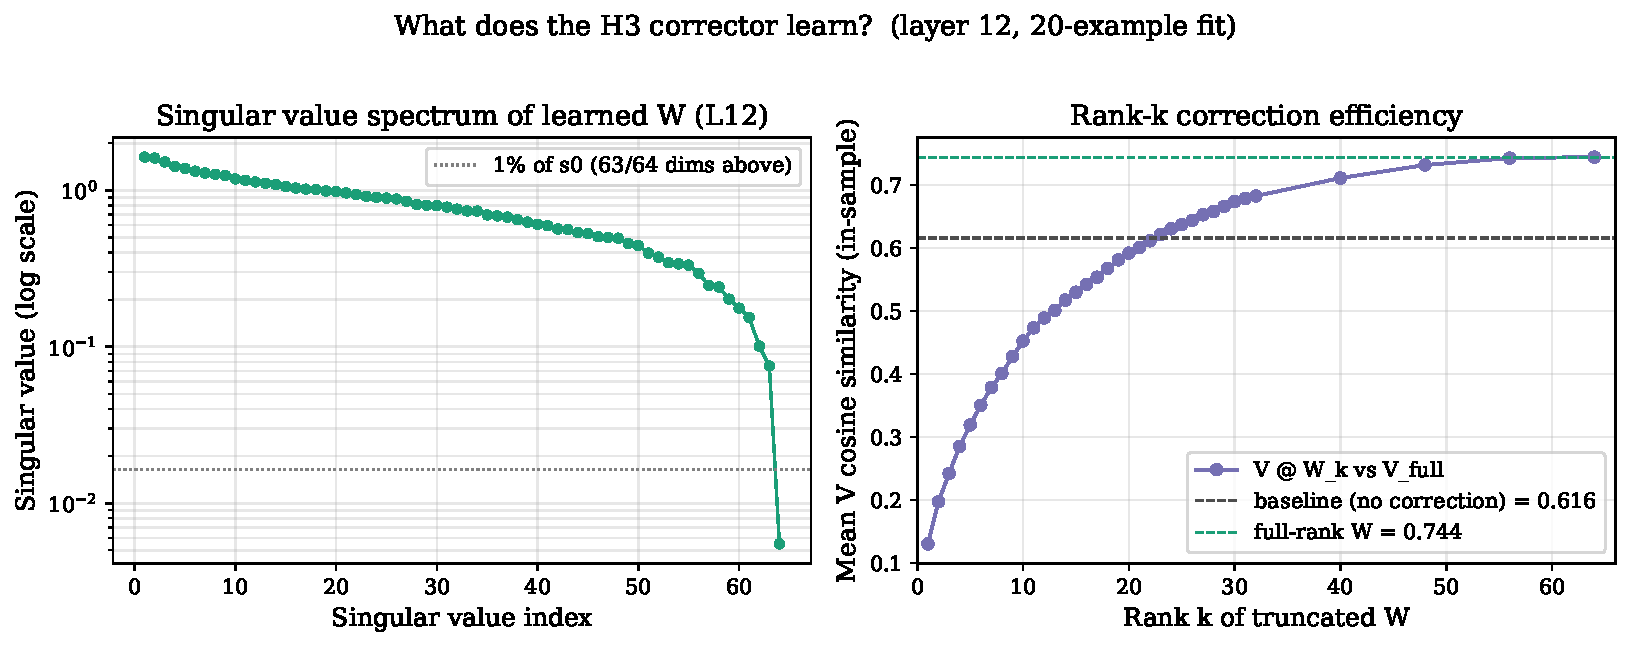
\includegraphics[width=\textwidth]{W_spectrum.pdf}
\caption{Left: singular values of the trained $64\times64$ corrector $W$ (log scale); the spectrum is nearly full-rank. Right: rank-$k$ truncated $W_k$ evaluated in-sample by mean $V$ cosine similarity. Gain relative to the un-corrected baseline (grey dashed) becomes positive only around $k \approx 22$, and reaches $90\%$ of the full-rank gain (green dashed) at $k = 48$.}
\label{fig:wspec}
\end{figure}

\subsection{Cost}\label{sec:cost}

Wall-clock measurements on CPU (median of five runs, $|B|=19$) are reported in Table~\ref{tab:cost}. Composition itself (M1, M2) is under $5\%$ of one $B$-prefill. The H3 correction adds approximately $0.34$ ms and $\sim 311{,}000$ FLOPs (a $64\times64$ matmul on $|B|\cdot H_{\mathrm{kv}} = 38$ rows), i.e.\ $\sim 0.0021\%$ of the estimated $\sim 14.85$ GFLOPs required for one $B$-prefill forward.

\begin{table}[t]
\centering
\caption{Wall-clock cost of composition on CPU, relative to a single $B$-prefill forward. Setup: Qwen-2.5-0.5B, CPU (single-thread PyTorch), $|B|=19$ tokens, $\mathrm{KV}_A$ and $\mathrm{KV}_B$ already computed and in memory (KV storage / transfer costs are not measured). H3 correction is a $64\times64$ matmul at a single layer. Numbers are the median of 5 runs.}
\label{tab:cost}
\begin{tabular}{lrr}
\toprule
Operation & Wall-clock (ms) & \% of prefill($B$) \\
\midrule
prefill($B$) baseline           & 344.9 & 100.00 \\
M1 naive concat                 &   3.1 &   0.91 \\
M2 RoPE-shift concat            &  14.1 &   4.08 \\
M4 naive + H3 correction        &   3.5 &   1.00 \\
M5 RoPE-shift + H3 correction   &  13.4 &   3.90 \\
\bottomrule
\end{tabular}
\end{table}

\begin{figure}[t]
\centering
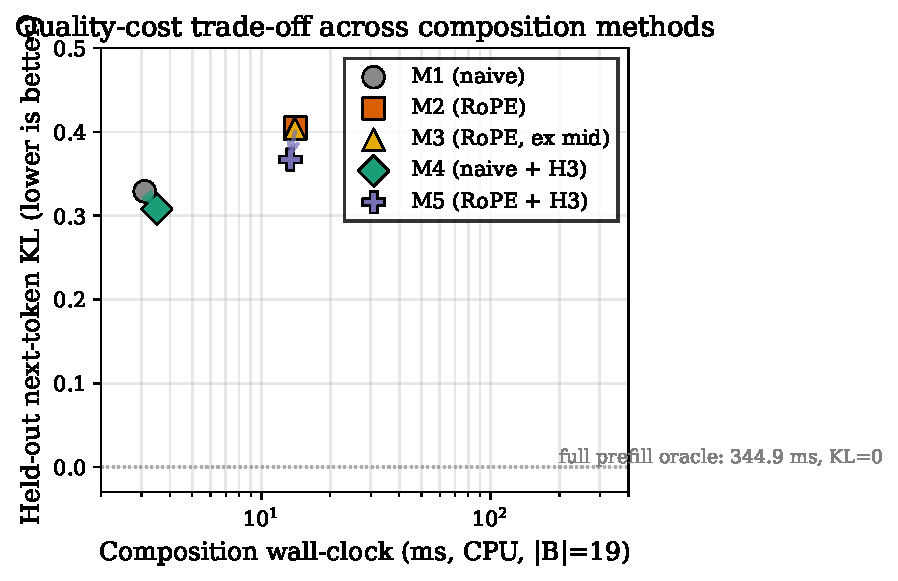
\includegraphics[width=\textwidth]{pareto.pdf}
\caption{Quality--cost trade-off across composition methods. Left: aggregate next-token KL under tokenization-aligned scoring (Table~\ref{tab:main}), sorted with the best on top; the dashed line at $0.578$ marks the (essentially overlapping) M1/M2 un-corrected baselines. The strongest single method is $M3$ (layer-selective RoPE-shift), followed by $M5$ (M2 + H3) and $M4$ (M1 + H3); $M2$ (full RoPE-shift) barely improves on $M1$ in aggregate. Right: composition wall-clock in the same method order (Table~\ref{tab:cost}), with a dashed reference at the full-prefill cost (345~ms). Setup: Qwen-2.5-0.5B, CPU, $|B|=19$, $\mathrm{KV}_A, \mathrm{KV}_B$ already computed and in memory.}
\label{fig:pareto}
\end{figure}

\section{Discussion}

Under a tokenization-aligned baseline, the aggregate held-out H3 reduction is $-1.7\%$ (M4 vs M1) and $-3.8\%$ (M5 vs M2). The single strongest method in aggregate is not $M5$ or $M4$ but $M3$, a purely rule-based layer-selective RoPE-shift ($-9.5\%$ over M2). These numbers are small in absolute terms; the primary contribution of the paper is the decomposition of composition error (Sections~\ref{sec:m2}, \ref{sec:interp}) and the structure of the analysis: RoPE-shift alone does not uniformly improve KL, but leaving the mid layers un-shifted does, consistent with the layer-wise cosine dip. The learned $W$ that closes part of the remaining gap does so through a nearly full-rank transformation of the value cache, not a small subspace.

Two qualitative findings we did not anticipate stand out:

\paragraph{Top-1 and KL move mostly together under aligned tokenization.} An earlier drift-affected version of this pipeline suggested a systematic pattern where M2 (RoPE-shift) improved top-1 agreement while worsening KL. Under tokenization-aligned scoring, the pattern is much weaker: M2 improves both top-1 and KL on \emph{independent} and \emph{conflicting}, and worsens both on \emph{cross-inferential}. On \emph{referential} the top-1 is tied at zero (the baseline is degenerate) so the metrics are not comparable. We keep both metrics in Table~\ref{tab:main} because they can in principle diverge, but the specific ``top-1 up, KL down'' story we reported earlier was partly a tokenization artifact.

\paragraph{RoPE-shift and H3 are complementary on the conflicting condition.} $M5$ (RoPE $+$ H3) achieves the strongest single-condition reduction on \emph{conflicting} ($0.639 \to 0.429$ held-out, roughly $-33\%$; top-1 agreement $1.00$), suggesting that on this condition the two error sources (position and cross-context) can be addressed in the same pipeline without interference. On the other three conditions the picture is more mixed: on \emph{cross-inferential} the un-corrected M1 is already close to the oracle and none of the shifts or corrections help; on \emph{referential} the baseline itself is degenerate.

\section{Limitations}

We are explicit about what this study does \emph{not} yet show.

\begin{itemize}[leftmargin=*]
    \item \textbf{Model scale.} Qwen-2.5-0.5B only. Larger models may exhibit different layer-wise divergence patterns, and their baselines are typically more reliable on referential and reasoning queries; on the current model, the baseline itself fails cross-inferential arithmetic in some examples, muddying KL comparisons.
    \item \textbf{Model family.} Only Qwen tested; different RoPE bases, GQA structures, or attention patterns in Llama, Mistral, or Gemma may respond differently.
    \item \textbf{Realistic workloads.} 20 hand-crafted controlled examples. RAG, long-context QA, and multi-turn dialogue are unexplored.
    \item \textbf{Sample size and leakage.} $n=5$ per condition; example templates share entity and structural patterns. A larger benchmark with entity, length, and template variation is a near-term follow-up.
    \item \textbf{Corrector expressivity.} A single target layer ($l^\star=12$) and a linear map. Whether an MLP, an $A$-context-conditional corrector, or a multi-layer application yields larger gains is untested.
    \item \textbf{Composition depth.} Only two prefixes. Chains ($A + B + C + \ldots$) are unexplored.
\end{itemize}

None of these blockers is fatal to the direction; each is the subject of a concrete follow-up experiment in the project's public repository.

\section{Conclusion}

We separately analyzed two conceptual error sources of independent-prefill KV composition -- a position component fixable by RoPE-shift, and a cross-context representation component that is not -- and showed on a $20$-example controlled benchmark that a single $64\times64$ linear map on the mid-layer value cache reduces held-out downstream next-token KL by $1.7\%$ (over naive concat) and $3.8\%$ (over RoPE-shift) in aggregate under a tokenization-aligned baseline. The gain is small in absolute terms, largest on the \emph{conflicting} condition, and driven by a nearly full-rank transformation of the value cache. The corrector adds approximately $0.34$ ms and $0.0021\%$ of the FLOPs of one $B$-prefill. Scaling the benchmark, reproducing on larger and more diverse models, an entity- or template-disjoint held-out split, and a direct comparison to CacheBlend~\citep{yao2024cacheblend} are the natural next steps.

\paragraph{Code and reproduction.} All code, data conditions, raw result logs, sanity checks, and cost measurements are released at \url{https://github.com/yunhyuk-mun/composable-kv} under an MIT license.

\bibliographystyle{plainnat}
\bibliography{references}

\appendix

\section{Pipeline sanity checks}\label{app:sanity}

We report four sanity checks against which every downstream number in this paper is measured. Numerical bounds are reported to make the noise floor of the composition pipeline explicit.

\begin{enumerate}[leftmargin=*]
    \item \textbf{Round-trip} (KL is preserved by cache injection). For every example $(A, B, Q)$ we tokenize once as $[A; B; Q]$ and compare next-token distribution of two routes: (i) $\mathrm{prefill}([A;B])$ followed by an incremental forward on $Q$ with the prefix cache; (ii) direct $\mathrm{prefill}([A;B;Q])$. Both routes must consume identical token ids to control for BPE boundary effects.
    Result: maximum KL across the 20 examples is $3.13\times10^{-7}$.
    \item \textbf{RoPE-shift(0)} is the identity map on $K$. Result: maximum $|K - R(0)K|$ over all 24 layers is $0.0$ (exact).
    \item \textbf{Determinism}: two independent prefill runs of the same input produce bitwise-identical $K$ and $V$. Result: exact.
    \item \textbf{Causal $A$-portion}: because the joint prefill is causal, tokens in $A$ cannot attend to $B$; their contribution to the joint cache should equal the $A$-alone cache. Result: maximum $|K^{(l)}_{\text{full}, :|A|} - K^{(l)}_A|$ is $1.53\times10^{-5}$, and similarly $5.25\times10^{-6}$ for $V$. This is at the expected float32 precision floor.
    \item \textbf{Tokenization boundary alignment.} We compare the token id sequence produced by $\mathrm{tokenize}(A) \Vert \mathrm{tokenize}(B) \Vert \mathrm{tokenize}(Q)$ against the sequence produced by $\mathrm{tokenize}(A + \text{`` ''} + B + Q)$. Result: 20/20 examples exhibit a boundary-length difference of $1$--$2$ tokens between the two constructions. \emph{Consequence.} An earlier version of this pipeline built the baseline from the re-tokenized joint string while the composition path used the separately-tokenized concatenation; that mismatch entered every reported KL number as a small BPE-boundary artifact. \emph{Fix.} We now enforce that the composition path and the from-scratch baseline consume the identical concatenated token id sequence $\mathrm{tokenize}(A) \Vert \mathrm{tokenize}(B) \Vert \mathrm{tokenize}(Q)$ in both \texttt{mve.py} and \texttt{h3\_holdout.py}. Every downstream number in Tables~\ref{tab:main}, \ref{tab:holdout}, and~\ref{tab:cost} is reported under this alignment. Aggregate H3 gains shrank from $6.4\%$/$9.4\%$ (drift-affected) to $1.7\%$/$3.8\%$ (aligned); the smaller aligned numbers are the ones our claims are stated in.
\end{enumerate}

Because the observed downstream method deltas (Table~\ref{tab:main}) are on the order of $10^{-2}$ KL, they are approximately $10^5$ times the round-trip noise floor, and their attribution to composition behavior (rather than injection artifacts) is safe under the tokenization-aligned pipeline.

\end{document}
